\section{Direct Visualization}

Model-based techniques are based on assumptions that limit their applicability to certain real world applications. Especially in diagnostic settings, where simplifying assumptions are not acceptable, it is essential to visualize the data directly "as it is". Direct Volume Rendering via GPU ray tracing, together with filtering and projection techniques is primarily employed for this purpose.

Volume Data is typically acquired via X-ray or magnetic resonance tomographic imaging techniques (CT, MR). To segment the vascular structures from the other tissue, so called "vesselness" filters that preserve only tubular structures can be used. A high vesselness for example may be defined as a situation where one of the three eigenvalues of the Hessian matrix (matrix of second derivatives) is considerably larger than the other two, indicating variance in one main direction. Other vesselness filter additionally employ entropy based filtering. Other tubular structures, like bones, are not reliable removed via such methods, however. In the case of angiography (CTA, MRA), i.e. the visualization of the vessels, an intravenous contrast agent is typically used. However, the intensities of structures enhanced via the contrast agent are often similar to the high intensitites resulting from bony structures. Thus, bones are typically removed via semi-automatic (where the user clicks at a structure) or automatic methods that involve region growing.

One of the main diagnostic tasks where DVR is employed is the detection of pathological conditions in vasculature, such as stenosis (narrowing of the vessel wall) or aneurisms (balloon-like bulges in the vessel wall) as well as obstructions from plaques or blood clots. An essential aspect in this regard is the choice of the transfer function, that maps intensity values sampled along rays in tracing to color and opacity values. Typically in DVR, these color and opacitiy values are accumulated, such that the contributions of occluded regions might not make it into the final image, since full opacity is already reached earler on the ray thus leaving to chance of the intensities farther away to reach the eye. Thus for example, in a 3D visualization the detection of pathological conditions that are surrounded by a lot of other tissue, may be difficult due to such occlusion.

\subsection*{Specialized Transfer Functions for 3D Views}

To provide a means of inspecting dense volumetric data in a 3D view more easily, intensity projection techniques are used. The most widely known technique in this context is Maximum Intensity Projection (MIP), which simply means that the maximum of all intesities sampled along a ray is assigned to its corresponding pixel. MIP allows for distant high-intensity structures, such as calcified plaques or stents, to "shine through" from arbitrary distances without being influenced by lower intensity tissues along the ray. Other projection techniques are Minimum Intensity Projection (MINIP), which may reveal soft plaques. Soft plaques consisting mainly of lipids are separated from the vessel lumen only by a thin fibrous cap, which is prone to rupture; blood clot formation around the rupture can lead to blocking of the artery. Average Intensity Projection is less commonly employed. 

Notably, there is one important limitation of these intensity projection techniques: There is a loss of depth information of the projected intensity values, as the accumulation of color and opacity along the ray is not given as in DVR. The user is thus required to rotate the view to get a proper understanding of the spatial structure via motion parallax.
Closest Vessel Projection, also known as Local MIP, uses the first local maximum in intensity above a user defined threshold. Thus, vessels of high intensity that are closer than the global maximum can be visualized as well, while low intensity structures still have no influence.

A more recent approach in the design of transfer functions, by Bruckner and Gr{\"o}ller~\cite{bruckner2009instant} combines the advantages both traditional DVR (depth perception via occlusion from opacity accumulation) as well as MIP (highlighting structures of high intensity even though they are occluded by structures of lower intensity). Their technique is called Maximum Intensity Difference Accumulation. The idea is to adjust the blending factor used in the accumulation of samples along the ray based on the change in the maximum intensity samples so far. As long as the maximum intensity is unchanged from previous samples, the last sample contributes fully with its opacity and color like in DVR. However if the intensity of the next sample is a new maximum, then the previous value (i.e. all that was accumulated before) is weighted less, leaving more opacity for the new maximum intensity to shine through, as seen in Figure~\ref{fig:midaRayProfiles}. Thus there is an accumulation, but local maxima are highlighted as well. 
\begin{figure}[htb]
  \centering
  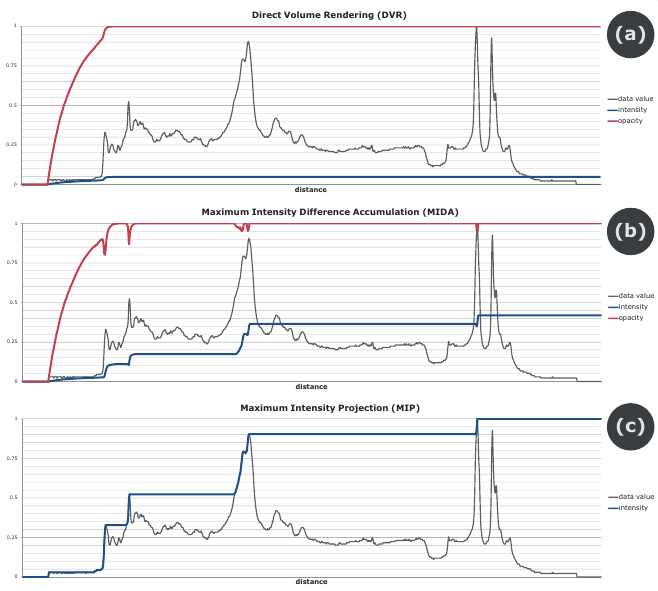
\includegraphics[width=0.45\textwidth]{mida_ray_profiles.png}
  \caption{\label{fig:midaRayProfiles} Ray profiles for DVR, MIDA and MIP.}
\end{figure}
Using a single control parameter, the user can switch between more accumulation (more like DVR) or more emphasis of maxima (more like MIP), as seen in Figure~\ref{fig:midaVasculature}. MIDA thus presents a unifying method of both traditional DVR and MIP via a simple extension.
Bruckner and Gr{\"o}ller also enhance the technique with gradient based shading, a common technique used in DVR, and weight the contribution of the shading by the magnitude of the gradient to avoid noise in homogenous regions.

\begin{figure*}[htb]
  \centering
  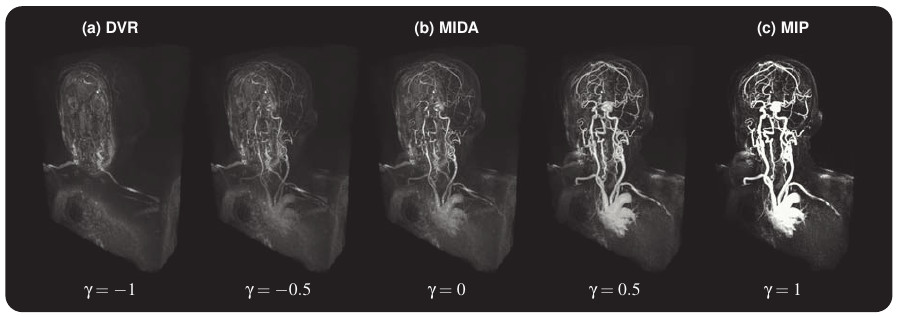
\includegraphics[width=1.0\textwidth]{mida_vasculature.jpg}
  \caption{\label{fig:midaVasculature} Maximum Intensity Difference Accumulation provides a technique that unifies both traditional DVR and MIP. Using a single control parameter, the user can switch between more accumulation (more like DVR) or more emphasis of maxima (more like MIP).}
\end{figure*}

While MIDA proves very useful for the visualization of vascular structures, it is still a very general technique. Other techniques are tailored more towards specific diagnostic tasks, such as the visual emphasis of pathological structures. Glasser et al.~\cite{glasser2010automatic} present a method that aids the quantitative evaluation of coronary artery plaque via specialized transfer functions that are automatically adjusted to fit the segmented artery data. Specifically, their approach aims to emphasize the vessel wall and its abnormalities, like hard and soft plaques or stents. Initially, a segmentation of the coronary arteries is performed. Then, the mean and standard deviation of both blood and vessel wall are computed. This is however not as straightforward as it may seem, due to non-uniform contrast agent accumulation and differing Hounsfield (HU) units. To overcome this limitation, the authors compute an intensity profile volume (IPV) for each artery branch. Each IPV is a stack of histograms computed radially from vessel centerline positions in its orthogonal planes, as seen in Figure~\ref{fig:glasserIPV}. These histograms are then used to determine the local mean and standard deviations for blood and vessel wall.
\begin{figure}[htb]
  \centering
  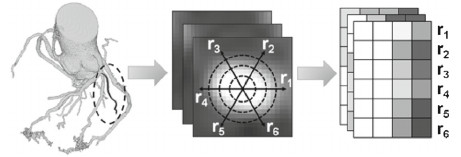
\includegraphics[width=0.45\textwidth]{glasser_intensity_profile_volume.jpg}
  \caption{\label{fig:glasserIPV} Computation of Intensity Profile Volumes to determine local blood and vessel wall intensity distribution of each branch.}
\end{figure}
The transfer function is designed in a way such that both the vessel wall and soft plaques as well as high intensity structures such as hard plaques are highlighted, as seen in Figure~\ref{fig:glasserTransferFunction}. The tresholds are set automatically corresponding to the computed local branch intensity distributions. Two thresholds, $S_3$ and $S_6$ can be adjusted by the user, determining the average vessel wall intensity and the threshold for hard plaque. Results can be seen in Figure~\ref{fig:glasserResult}.
\begin{figure}[htb]
  \centering
  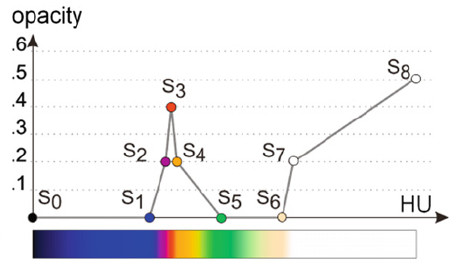
\includegraphics[width=0.45\textwidth]{glasser_transfer_function.jpg}
  \caption{\label{fig:glasserTransferFunction} A transfer function that highlights vessel wall and hard plaques, automatically adjusted to local intensity distribution.}
\end{figure}
\begin{figure}[htb]
  \centering
  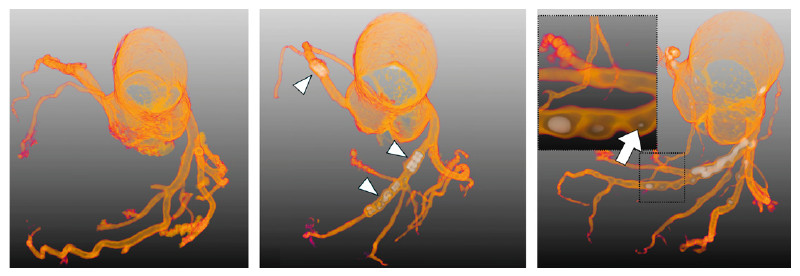
\includegraphics[width=0.45\textwidth]{glasser_result.jpg}
  \caption{\label{fig:glasserResult} Results of the automatically adjusted transfer functions by Glasser et al.~\cite{glasser2010automatic} to highlight vessel wall and abnormalities such as plaques or stents.}
\end{figure}

\subsection*{Rotation Independent Projection Techniques for 2D Views}

When it comes to the inspection of volumetric data via 2D views, other projection techniques are used, to ensure visibility of possibly occluded vascular structures. A widely used technique is Curved Planar Reformation (CPR), of which the basic three types are projection CPR, stretched CPR and straightened CPR. Two more recent improvements to CPR are discussed in the following.

Mistelbauer et al.~\cite{mistelbauer2010automated} present a technique called Centerline Reformations (CR), that aims at simultaneously visualizing the inside (lumen) of multiple arbitrarily oriented vessels in CPR. Using CPR, the vessel lumen may be inspected by defining a curved cut along the vessel centerline. However this is only possible for single vessels, not for the whole vessel tree. In CR, first the vessel centerlines and radii are extracted from the volume via scale-space feature detection: Contrast-enhanced data is filtered using a Hessian-based vesselness filter followed by a segmentation based on Hysteresis thresholding as used by the Canny edge detector. The Hysteresis thresholding uses two threshold values to ensure continuous edges without gaps, when the data fluctuates: When the data is below the lower threshold, it is rejected, but if it is inbetween the thresholds, it is still accepted if it is connected to a value above the higher threshold. The union of the resulting binary volumes is then used to determine the radius via the Hessian scale with maximum response, and the centerlines are extracted using skeletonization via a thinning technique. Then, a graph representation of the vessel tree is additionally computed to allow for user interaction such as selection etc. The vessel lumen itself is then rendered using wavefront propagation from the vessel centerline, which is based on the Fast Marching Method (FMM). The initial wavefronts are simply arrays of pixels along the centerline from orthogonal projection of the volume to the 2D view. For each pixel additional data is stored: the corresponding graph edge, voxel, pixel type (vessel, halo, background) vessel radius as well as the depth and arc-length (distance of pixel in projected space to the first pixel of the centerline). The wavefronts (arrays of pixel data) are then propagated to neighboring pixels orthogonal to the centerline until the radius is reached assigning the corresponding projected volume data along the way, then optionally continuing by drawing a halo, as seen in Figure~\ref{fig:crWavefrontPropagation}. For background pixels, traditional MIP or MIDA can be used.
\begin{figure}[htb]
  \centering
  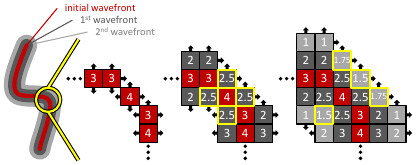
\includegraphics[width=0.45\textwidth]{cr_wavefront_propagation.jpg}
  \caption{\label{fig:crWavefrontPropagation} Results of the automatically adjusted transfer functions by Glasser et al.~\cite{glasser2010automatic} to highlight vessel wall and abnormalities such as plaques or stents.}
\end{figure}
Since vessels may overlap, the wavefront propagation requires a comparison of the currently stored pixel buffer at closest depth with the current vessel wavefront. Since a wavefront may also collide with itself leading to ambiguities in value assignment, the arc length, i.e. position along the centerline of pixels is also propagated and used for this decision.

A different technique also presented by Mistelbauer et al.~\cite{mistelbauer2013vessel} is called Curvicircular Feature Aggregation (CFA). The idea of CFA is to reduce the amount of user interaction required when working with CPR angiography data, i.e. rotation around the vessel centerline to inspect it from all directions. CFA provides a single image where aggregated intensities around the vessel centerline are depicted. This is done by sampling intensities in circular rays around the assumed vessel centerline and aggregating the samples with MIP or MINIP, as shown in Figure~\ref{fig:ctaOverview}. Samples may be placed along the circular rays either at costant angles or constant arc-lengths, the latter providing more samples and thus also more computational overhead. The resulting image is split in two parts: The centerline is straightened and placed vertically from top to bottom, separating the image in left and right side. Thus the vertical dimension relates to the position along the centerline. The horizontal distance from the centerline corresponds to the radius of the circular rays: Each pixel at certain horizontal distance from the centerline shows the result of the aggregation around a circular ray with the corresponding radius. On the left side, MIP is used for the aggregation (or rather, projection), on the right side MINIP is used.
\begin{figure}[htb]
  \centering
  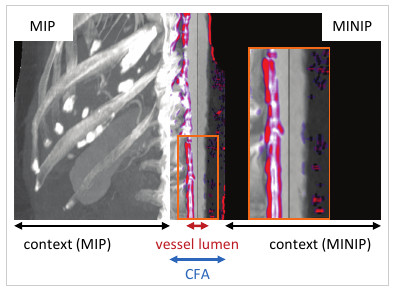
\includegraphics[width=0.45\textwidth]{cta_result.jpg}
  \caption{\label{fig:ctaResult} }
\end{figure}
For radii that by far exceed the vessel radius, there is no point in doing the curvicircular feature aggregation. Instead, standard MIP and MINIP projections from a single direction are shown in pixels beyond a certain horizontal distance from the centerline, to use the image space for context, as seen in Figure~\ref{fig:ctaResult}.
\begin{figure*}[htb]
  \centering
  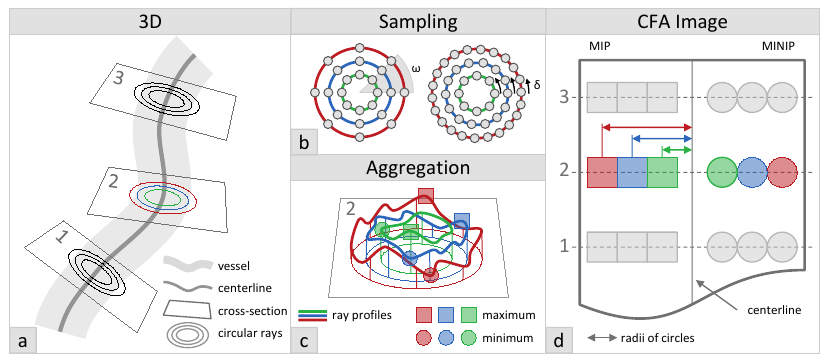
\includegraphics[width=1.0\textwidth]{cta_overview.png}
  \caption{\label{fig:ctaOverview} }
\end{figure*}
Another feature of the technique is to display a measure of stability of the centerline estimation at each given point along the vessel. This is done by computing the variance of values sampled in the neighborhood of each centerline point, to determine the local uniformity around it. If there is a high variance, i.e. low stability, the centerline estimation may deviate from the actual centerline in the vessel volume data. The variance is mapped to a color range from red to blue, red meaning higher variance, i.e. less stability.


\subsection*{Depth Cues for Direct Volume Rendering}

Kersten-Oertel et al.~\cite{kersten2014evaluation} provide an extensive evaluation of monoscopic depth cues used in real time renderings of 3D angiographic data. The fast and accurate perception of relative depth and structure of overlapping vessels is essential for intraoperative guidance, where surgeons often have little time to make important decisions. The study compares the effectiveness of fog (mapping of depth to saturation), pseudo-chromadepth (mapping depth to color from red to blue), kinetic depth (depth by continuous rotation around the structure), edges as well as stereopsis (using shutter glasses). 

The authors note a number of limitations of the operating room. Interaction with the data (which can provide depth cues via the parallax effect apparent from the movement) are typically not possible due to the need for sterility. The surgeon typically needs to verbally instruct an assistant to do the interaction via mouse and keyboard, thus making real time interaction unfeasable. Moreover, head mounted displays to provide stereopsis are typically not acceptable due to operating room constraints. Thus monoscopic depth cues play an important role.

The study shows results of experiments where participants had to state which of two vessels is closer, for each of the depth cues and with all possibly influencing parameters randomized.
In results both with novices unexperienced in vasculature as well as expert neurosurgeons, both the fog and pseudo-chromadepth cues gave best results both in time and correctness. Accordint to the authors, the short time needed to provide the correct result indicates that little additional processing is required, reducing the perception of depth to a comparison of saturation or hue. The kinetic depth cue proved unreliable and prone to confusion of front and back due to orthographic projection used in clinical settings. The stereoscopic cue interestingly did not yield better results, indicating that their benefit is task dependent. The edge cue was beneficial for expert neurosurgeons, who used the edge information to trace the path of vessels to determine which was closer.
